\documentclass{article}

\usepackage[T1]{fontenc}
\usepackage[utf8]{inputenc}
\usepackage{times}

\usepackage[font=small,labelfont=bf,tableposition=top]{caption}
\usepackage{graphicx}
\usepackage{natbib} 

\usepackage{amsmath}
\usepackage{amsfonts}
\usepackage{amssymb}
\usepackage{color, soul}
\usepackage{hyperref}
\usepackage{algorithmicx}
\usepackage{algpseudocode}
\usepackage{subfigure}
\usepackage{stmaryrd}

\renewcommand{\vec}[1]{\boldsymbol{{#1}}} 
\newcommand{\duesoon}[1]{{\sethlcolor{green}\hl{#1}}}
\usepackage{mathrsfs}


\newtheorem{theorem}{Theorem}
\newtheorem{acknowledgement}[theorem]{Acknowledgement}
\newtheorem{algorithm}[theorem]{Algorithm}
\newtheorem{axiom}[theorem]{Axiom}
\newtheorem{case}[theorem]{Case}
\newtheorem{claim}[theorem]{Claim}
\newtheorem{conclusion}[theorem]{Conclusion}
\newtheorem{condition}[theorem]{Condition}
\newtheorem{conjecture}[theorem]{Conjecture}
\newtheorem{corollary}[theorem]{Corollary}
\newtheorem{criterion}[theorem]{Criterion}
\newtheorem{definition}[theorem]{Definition}
\newtheorem{example}[theorem]{Example}
\newtheorem{exercise}[theorem]{Exercise}
\newtheorem{lemma}[theorem]{Lemma}
\newtheorem{notation}[theorem]{Notation}
\newtheorem{problem}[theorem]{Problem}
\newtheorem{proposition}[theorem]{Proposition}
\newtheorem{remark}[theorem]{Remark}
\newtheorem{solution}[theorem]{Solution}
\newtheorem{summary}[theorem]{Summary}
\newenvironment{proof}[1][Proof]{\textbf{#1.} }{\ \rule{0.5em}{0.5em}}

\newtheorem{guess}{Definition}
\newcommand{\comment}[1] {}
\newcommand{\Norder} {N}
\newcommand{\order}{\mathcal{O}}
\newcommand{\Npoints} {N_p}
\newcommand{\Nfaces} {N_{f}}
\newcommand{\Nelements} {N_e}

\newcommand{\eps}{\varepsilon}
\newcommand{\Dweak}{\wt{D}}
\newcommand{\diff}[2] {\frac{\partial #1}{\partial #2}}
\newcommand{\dxx}[2] {\frac{\partial^2 #1}{\partial {#2}^2}}
\newcommand{\difft}[2] {\frac{d #1}{d #2}}
\newcommand{\dxxt}[2] {\frac{d^2 #1}{d {#2}^2}}
\newcommand{\lagrange}[1] {\frac{d #1}{dt}}
\newcommand{\lebesgue}{\parallel I \parallel}
\newcommand{\polysp}{\mathcal{P}_N}
\newcommand{\laplacian}{\nabla^2}
\newcommand{\divergence}{\nabla \cdot}
\newcommand{\inte}{\int_{\mbox{\footnotesize ${\Omega_e}$}}}
\newcommand{\intb}{\int_{\mbox{\footnotesize ${\Gamma_e}$}}}
\newcommand{\intce}{\int_{\mbox{\footnotesize ${\widehat{\Omega}_e}$}}}
\newcommand{\intcb}{\int_{\mbox{\footnotesize ${\widehat{\Gamma}_e}$}}}
\newcommand{\intg}{\int_{\mbox{\footnotesize ${\Omega}$}}}
\newcommand{\intgb}{\int_{\mbox{\footnotesize ${\Gamma}$}}}
\newcommand{\intv}{\int_{\mbox{\footnotesize ${\sigma}$}}}
\newcommand{\sumv}{\sum_{K=1}^{N_{\mathrm{lev}}}}
\newcommand{\sumk}{\sum_{L=1}^{K}}
\newcommand{\sumN}{\sum_{i=1}^{N+1}}
\newcommand{\half}{\frac{1}{2}}
\newcommand{\inti}{\int_{\mbox{\footnotesize\sf I}}}
\newcommand{\intbd}{\oint_{\mbox{\footnotesize ${\delta}$\sf D}}}
\newcommand{\intbi}{\oint_{\mbox{\footnotesize ${\delta}$\sf I}}}
\newcommand{\ldnorm}[1]{\left\| #1 \right\|_{\mbox{\footnotesize \sf D}} }
\newcommand{\lonorm}[1]{\left\| #1 \right\|_{\Omega}}
\newcommand{\spc}[1]{\mbox{\sf #1}}
\newcommand{\ope}[1]{{\cal #1}}
\newcommand{\mt}[1]{{\rm #1}}
\newcommand{\dis}{\displaystyle}
\newcommand{\ve}{\varepsilon}
\newcommand{\ov}{\overline}
\newcommand{\wt}{\widetilde}
\newcommand{\wh}{\widehat}
\newcommand{\Dhat}{\widehat{D}}
\newcommand{\be}{\begin{equation}}
\newcommand{\ee}{\end{equation}}
\newcommand{\bea}{\begin{eqnarray*}}
\newcommand{\eea}{\end{eqnarray*}}
\newcommand{\Jace}{J^{(e)}}
\newcommand{\Jacl}{J^{(l)}}
\def\bepsilon{\mbox{\boldmath $\epsilon $}}
\def\bpsi{\mbox{\boldmath $\psi $}}
\def\bphi{\mbox{\boldmath $\phi $}}
\def\bmu{\mbox{\boldmath $\mu $}}
\def\Et{ \tilde{E} }
\def\Ht{ \tilde{H} }
\def\sdot{ \dot{\sigma} }

\newcommand{\fstar}{f^{(*)}}

\DeclareMathOperator{\Span}{span}
\DeclareMathOperator{\Dim}{dim}

\newcommand{\polyquad}{\mathcal{Q}_{N}}
\newcommand{\polyP}{\mathcal{P}_{N}}
\newcommand{\polyPnpm}{\mathcal{P}_{(N+M)}}
\newcommand{\polyPd}{\mathcal{P}_{d}}
\newcommand{\polyPnm}{\mathcal{P}_{N,M}}
\newcommand{\polyPn}{\mathcal{P}_{N,0}}
\newcommand{\transpose}{^{\mathcal{T}}}

\newcommand{\vecQ}{\vec{Q}}
\newcommand{\vecQe}{\vec{Q}^{(e)}}
\newcommand{\vecFe}{\vec{\mathcal{F}}^{(e)}}
\newcommand{\statevec}{\vec{Y}}
\newcommand{\statevecN}{\vec{Y}_N^{(e)}}
\newcommand{\statestage}{\vec{\mathcal{Y}}}
\newcommand{\Ftensor}{\vec{F}(\qvector)}
\newcommand{\FtensorN}{\vec{F}\left( \qvectorN \right)}
\newcommand{\FtensorStar}{\vec{F}\left( \qvector_N^{(e,k)} \right)}
\newcommand{\Svector}{S(\qvector)}
\newcommand{\SvectorN}{S \left( \qvectorN \right)}
\newcommand{\qref}{\vec{q}_0}
\newcommand{\qvectorb}{\vec{q}_b}
\newcommand{\qtt}{\vec{q}_{tt}}
\newcommand{\qhat}{\widehat{\vec{q}}}
\newcommand{\qhatb}{\widehat{\vec{q}}_b}
\newcommand{\qelem}{q^{(e)}}
\newcommand{\rhoref}{\rho_0}
\newcommand{\piref}{\pi_0}
\newcommand{\Thetaref}{\Theta_0}
\newcommand{\Gref}{G_0}
\newcommand{\Tref}{T_0}
\newcommand{\thetaref}{\theta_0}
\newcommand{\Pref}{{P}_0}
\newcommand{\Eref}{{E}_0}
\newcommand{\Href}{{h}_0}
\newcommand{\rhohat}{\widehat{\rho}}
\newcommand{\pihat}{\widehat{\pi}}
\newcommand{\Phat}{\widehat{P}}
\newcommand{\uvechat}{\widehat{{\mbox{\boldmath$u$\unboldmath}}}}
\newcommand{\uhathat}{\widehat{\widehat{{\mbox{\boldmath$u$\unboldmath}}}}}
\newcommand{\Uhat}{\widehat{{\mbox{\boldmath$U$\unboldmath}}}}
\newcommand{\Uhathat}{\widehat{\widehat{{\mbox{\boldmath$U$\unboldmath}}}}}
\newcommand{\thetahat}{\widehat{\theta}}
\newcommand{\Thetahat}{\widehat{\Theta}}
\newcommand{\Ehat}{\widehat{E}}
\newcommand{\uhat}{\widehat{u}}
\newcommand{\vhat}{\widehat{v}}
\newcommand{\what}{\widehat{w}}
\newcommand{\pitt}{\pi_{tt}}
\newcommand{\rhott}{\rho_{tt}}
\newcommand{\Ett}{E_{tt}}
\newcommand{\Utt}{\vec{U}_{tt}}
\newcommand{\uvectt}{\vec{u}_{tt}}
\newcommand{\utt}{u_{tt}}
\newcommand{\vtt}{v_{tt}}
\newcommand{\wtt}{w_{tt}}
\newcommand{\Ptt}{P_{tt}}
\newcommand{\vecPtt}{\vec{P}_{tt}}
\newcommand{\Thetatt}{\Theta_{tt}}
\newcommand{\thetatt}{\theta_{tt}}
%Projector Matrices
\newcommand{\projmatrix}{\vec{\mathcal{P}}}
\newcommand{\qmatrix}{\vec{\mathcal{Q}}}
\newcommand{\pcmatrix}{\vec{\mathcal{P}}_C}
\newcommand{\Cmatrix}{\left(\vec{\mathcal{C}}^{(e,f)}\right)\transpose}
\newcommand{\Dmatrix}{\vec{D}^{(e)}}
\newcommand{\Dwmatrix}{\wt{\vec{D}}^{(e)}}
\newcommand{\Mmatrix}{M^{(e)}}
\newcommand{\Fmatrix}{\vec{F}^{(e,l)}}
\newcommand{\Gmatrix}{\mathcal{G}}
\newcommand{\Umatrix}{\mathcal{U}^{(e,f)}}
\newcommand{\amatrix}{\vec{\mathcal{A}}}
\newcommand{\rmatrix}{\vec{\mathcal{R}}}
%Vectors
\newcommand{\nvector}{\wh{\vec{n}}_{\Gamma}}
\newcommand{\nhat}{\wh{\vec{n}}}
\newcommand{\ivector}{\wh{\vec{i}}}
\newcommand{\jvector}{\wh{\vec{j}}}
\newcommand{\kvector}{\wh{\vec{k}}}
\newcommand{\rvector}{\wh{\vec{r}}}
\newcommand{\svector}{\wh{\vec{s}}}
\newcommand{\tvector}{\wh{\vec{t}}}
\newcommand{\vvector}{\wh{\vec{v}}}
\newcommand{\Qvector}{\vec{Q}}
%Vectors
\newcommand{\ur}{{u}^{(r)}}
\newcommand{\us}{{u}^{(s)}}
\newcommand{\ut}{{u}^{(t)}}
\newcommand{\urtt}{{u}_{tt}^{(r)}}
\newcommand{\ustt}{{u}_{tt}^{(s)}}
\newcommand{\uttt}{{u}_{tt}^{(t)}}
\newcommand{\urhat}{\widehat{u}^{(r)}}
\newcommand{\ushat}{\widehat{u}^{(s)}}
\newcommand{\uthat}{\widehat{u}^{(t)}}
%Other Operators
\newcommand{\grad}{\vec{\nabla}}
\newcommand{\Grad}{\vec{\nabla}}
\newcommand{\Dskew}{\mathcal{D}}

\def\bepsilon{\mbox{\boldmath $\epsilon $}}
\def\bpsi{\mbox{\boldmath $\psi $}}
\def\bphi{\mbox{\boldmath $\phi $}}
\def\bmu{\mbox{\boldmath $\mu $}}
\def\Et{ \tilde{E} }
\def\Ht{ \tilde{H} }
\def\sdot{ \dot{\sigma} }
%\renewcommand{\thetable}{\Roman{table}}
%\renewcommand{\thefigure}{\arabic{figure}}

%\DeclareMathOperator{\Span}{span}
%\DeclareMathOperator{\Dim}{dim}

%Editing Commands
\newcommand{\here}{ \textcolor{red}{YOU ARE HERE}}

%Time-Integration
\newcommand{\dt}{{\Delta t}}
\newcommand\ST{\rule[-0.75em]{0pt}{2em}}
\newcommand{\Sfunction}{\mathcal{S}}
\newcommand{\Lfunction}{\mathcal{L}}
\newcommand{\Nfunction}{\mathcal{N}}

%DG Operators
\newcommand{\average}[1]{ \left\{ #1 \right\} }
\newcommand{\jump}[1]{ \llbracket #1 \rrbracket }

%HDG Matrices
\newcommand{\CCmatrix}{\mathcal{C}^{(e,k)}}
\newcommand{\Jmatrix}{\mathcal{J}^{(e,k)}}
\newcommand{\DDmatrix}{\wt{D}^{(e)}}
\newcommand{\SSvector}{\mathcal{S}(q)}
\newcommand{\cghdg}{cg\underline{\hspace{0.15cm}}to\underline{\hspace{0.15cm}}hdg}
%\newcommand{\ul}{\underline{\hspace{0.15cm}}}
\newcommand{\RRmatrix}{\mathcal{R}}

%Clima specific variables
\newcommand{\etotal}{e^{\mathrm{tot}}}
\newcommand{\Etotal}{E^{\mathrm{tot}}}
\newcommand{\Fvector}{\vec{\mathcal{F}}}
\newcommand{\Pvector}{\vec{\mathcal{P}}}
\newcommand{\Fadv}{\vec{\mathcal{F}}^{\mathrm{adv}}}
\newcommand{\Fndf}{\vec{\mathcal{F}}^{\mathrm{ndf}}}
\newcommand{\Fdiff}{\vec{\mathcal{F}}^{\mathrm{diff}}}
\newcommand{\Tvector}{\vec{\mathcal{T}}}
\newcommand{\Source}{\vec{\mathcal{S}}}

\newcommand{\fxg}[1]{\textcolor{cyan}{FXG: #1}}



\title{Design Document for the CLIMA Land Model} 
\author{ }
      
\begin{document}
      
\maketitle
\tableofcontents

\section{Introduction}\label{s:introduction}

This document highlights the design specifications for the land model (CLIMA-land) that is part of the Climate Machine (CLIMA). The model will be designed to run both in standalone mode (e.g., driven by reanalysis data) and coupled to the atmosphere. Because it will be part of a climate model, conservation of energy, water and carbon are essential, both within the land model and for the exchanges with the atmosphere. We will also leave the treatment of atmospheric fluxes (e.g., even within canopies) to the atmosphere model, so that all turbulent fluxes are dealt with consistently within one model component, and that the land model can also be run at large-eddy simulation resolutions, where, e.g., trees and the air flow around them become explicitly resolved. 

The individual components of the land model will be developed in a modular fashion, but with consistent interactions. For example, the canopy model will interact with the soil model through source/sink terms representing processes such as water uptake by roots, and it will interact with turbulent fluxes in the atmospheric near-surface layer, for example, through exchange of momentum, energy, and water. 

The biophysical part of the land model consists principally of components for soil, snow, and plants.
\subsection{Interfaces between land modules}

The following section provides a higher-level description of the CliMA land model modules and the associated dependencies. Equations are provided in subsequent sections of this document

\newpage
\vfill

\begin{figure}[]
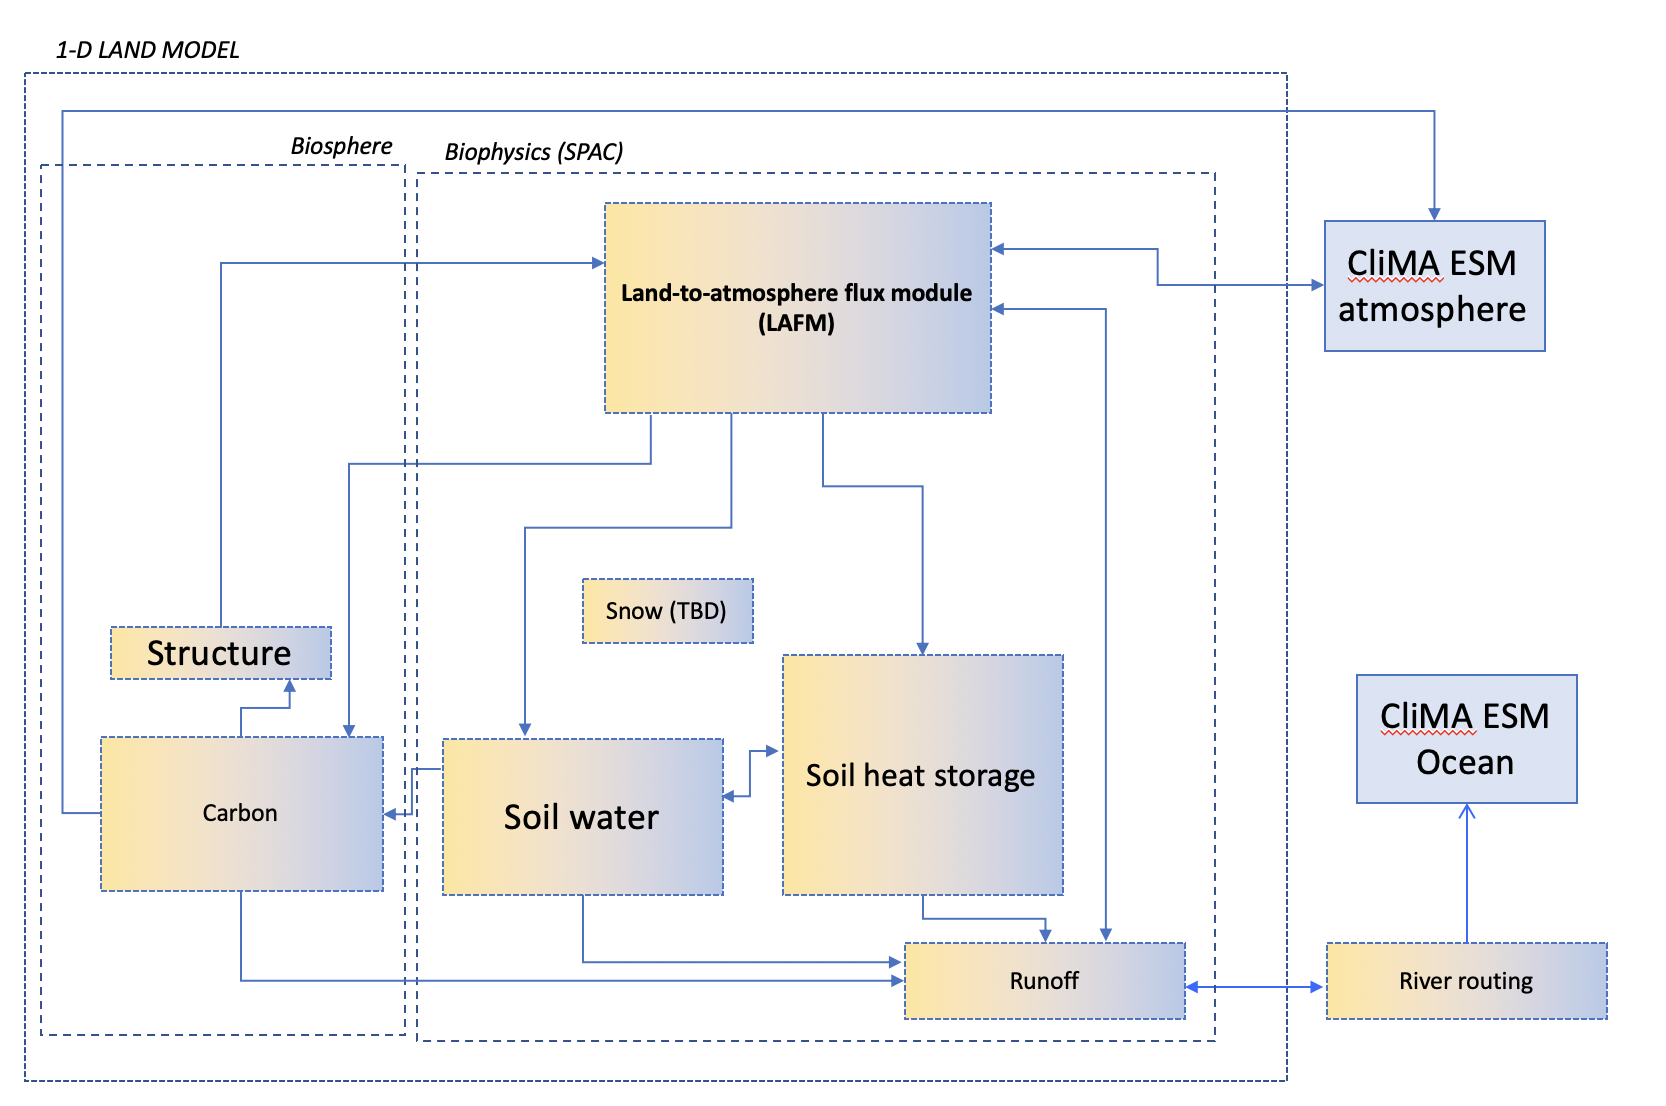
\includegraphics[width=10cm,height=10cm,keepaspectratio]{CLIMA-land/LM_figures/JPLCLIMA_LM_DESIGN_20191115.png}
\caption{Schematic of land model modules and internal + external dependencies. [ALL: please comment + suggest improvements; Pierre's comment: SPAC should include all biophysics, re-name/re-arrange/simmplify boxes]}
\end{figure}
% Please add the following required packages to your document preamble:
% \usepackage{graphicx}
\begin{table}[]
\resizebox{\textwidth}{!}{%
\begin{tabular}{|l|l|l|l|}
\hline
Module [code]         & Input requirements [From]                                                                & Output requirements                                                       & Module requirements                      \\ \hline
Carbon [C]            & \begin{tabular}[c]{@{}l@{}}GPP [F], \\ Soil water profile [W], \\ Soil temperature profile [E]\end{tabular}                                                               & \begin{tabular}[c]{@{}l@{}}Carbon states\\ (Biomass, inc. foliar, roots, wood;\\ Dead organic C) \\ Carbon fluxes \\ (respiration, disturbance fluxes)\end{tabular} & \begin{tabular}[c]{@{}l@{}}The carbon module will calculate \\ internal land biosphere carbon transfers \\ (allocation, mortality, mineralization), \\ and gross land-atmosphere C fluxes \\ (respiration, fires)\end{tabular} \\ \hline

Structure [S]         & Biomass [C]                                                             & \begin{tabular}[c]{@{}l@{}}Biophysical states:\\ Canopy height, Chlorophyll, \\Root profile, LMA\end{tabular}                                                        &                                                                   \\ \hline
Soil water [H]        & \begin{tabular}[c]{@{}l@{}}Soil freeze/Thaw state [E] \\ Precipitation [A]\\ Evaporation [F], \\ Transpiration (vertically resolved), \\ root profile [S]\end{tabular} &
\begin{tabular}[c]{@{}l@{}}
Vertical soil water states\\Soil water fluxes\\Runoff\end{tabular}                                                                                                                  & \begin{tabular}[c]{@{}l@{}}Module will calculate vertical \\ water flow in soil Darcy’s law, \\ Richards equations, hydraulic \\redistribution,  runoff, etc.\end{tabular}                                                     \\ \hline
Soil heat storage [E] & Soil water [H], Precip. temp [A]


& 
\begin{tabular}[c]{@{}l@{}}
Vertical temperature profile\\
Runoff temperature       \end{tabular}                                               &                                                                                                \\ \hline
%%%%%%(SPAC-Flux)%%%%%
\begin{tabular}[c]{@{}l@{}}
Land-to-atmosphere\\ fluxes [F]  \\
(previously SPAC-Flux)

\end{tabular}

        & \begin{tabular}[c]{@{}l@{}}Atmospheric variables [A], \\ Biophysical states[S], \\ Soil water profile [H], \\ Soil energy profile [E],\end{tabular}                   & \begin{tabular}[c]{@{}l@{}}Land-surface Fluxes\\ GPP, evapotranspiration, H, $\lambda$E, L↑, S↑ \end{tabular}                                 & 

\begin{tabular}[c]{@{}l@{}} Canopy P interception\\ Radiative transfer in canopy     \end{tabular}                                                        \\ \hline

River routing [R]        & \begin{tabular}[c]{@{}l@{}} Soil runoff [H], \\ CliMA Ocean [O] \end{tabular}                             & \begin{tabular}[c]{@{}l@{}} River Discharge\end{tabular}                                             &                                     \\ \hline \hline \hline


CliMA Atmosphere [A]        & \begin{tabular}[c]{@{}l@{}}Land surface fluxes [F], \\ Land biosphere fluxes [C]\end{tabular}                             & \begin{tabular}[c]{@{}l@{}}Atmospheric variables [for land]\\ L↓, S↓, precip, temperature, humidity,\end{tabular}                                             &                                     \\ \hline

CliMA Ocean [O]        & \begin{tabular}[c]{@{}l@{}}River discharge [R] \end{tabular}                             & \begin{tabular}[c]{@{}l@{}} Ocean variables (for land) Sea Level\end{tabular}                                             &                                     \\ \hline

\end{tabular}%
}
\caption{\label{tab:LM-modules}Summary of module input, output & functional requirements. Comprehensive list of module inputs, outputs and equations are included in subsequent sections. [MISSING: snow module and associated dependencies. Ensure consistency with rest of CliMA framework]}
\end{table}
\vfill
\clearpage

\section{Soil}

\textcolor{blue}{Yujie's comments. (1) In the heat equation, the heat transfer caused by water mass flow is not considered, and it is better to add a mass flow component, i.e. $\dfrac{\delta (C_s T_s)}{\delta t} = \dfrac{\delta \lambda_s}{\delta z} \dfrac{\delta T_s}{\delta z} + \rho_w c_w S_{in} \dfrac{\delta T_{in}}{\delta t} - \rho_w c_w S_{out} \dfrac{\delta T_{out}}{\delta t}$. (2) In the soil moisture equations, it is not clearly stated that soil hydraulic conductivity and soil water content are temperature dependent. Consider the impacts from temperature on (i) viscosity of water and (ii) surface tension of water. And maybe more.}

\subsection{Heat equation}

\textit{AAbloom comments and changes:  (i) define C in terms of $c_s$ and $\rho_s$--and their dependencies on $\theta$--in "soil heat capacity" section, and (ii) define eq. 1 in terms of volumetric heat capacity.}
\\

In the soil, heat follows a 1D vertical heat diffusion:
\begin{equation}
     \frac{\partial (C_s T_s) }{\partial t} = \frac{\partial }{\partial z}\lambda_s \frac{\partial T_s }{\partial z}
\end{equation}
where $C_s$--the volumetric heat capacity--is the product of soil density and specific heat capacity, i.e.  $C_s = \rho_s c_s$, and are defined in subsequent sections), and $\lambda_{s}$ is the thermal conductivity of the soil; both $\lambda_{s}$ and $C_s$ are functions of the soil moisture content, $\theta$. Note that the diffusion coefficient ($\alpha = \lambda_s/C_s$) has much less moisture dependence because of a compensation of the dependence between $\lambda_s$ and $C_s$.

\subsubsection{Soil heat capacity ($C_s$)}

\textit{AABloom comments and changes: 
\\
- Account for dry soil heat capacity + water heat capacity separately to account for phase change
\\
- Introduce fraction of frozen water (e.g. $f_\phi$) to account for this. I *think* this is already defined in eq. form in Marcos Longo's latex doc
\\
- Still need clear definition for $rho_s$, and clarification of whether it need be water dependent, or whether its the dry density (and therefore water is independently accounted for)}
//

*Elias's attempt, from Bonan book*

The heat capacity of the soil is (considering heat of the air to be negligible):
\begin{equation}
c_s = (1- \theta_{sat} ) c_{\rm solid} + (\theta_{liquid}) c_{\rm water} + (\theta_{ice}) c_{\rm ice}
\end{equation}
where the heat capacity of soil is $c_{\rm solids}$ = 1.926 MJ m$^{-3}$ K$^{-1}$, of water is $c_{\rm water}$ = 4.19 MJ m$^{-3}$ K$^{-1}$, and of ice is $c_{\rm ice}$ = 1.94 MJ m$^{-3}$ K$^{-1}$. 

\subsubsection{Thermal Conductivity ($\lambda_s$)}
*Elias's attempt, from Bonan book. Pierre: this is the same as CLM - we should just cite the appropriate ref. Farouki 1981*

Soil thermal conductivity is assumed to depend on soil water content:
\begin{equation}
\lambda_s = K_e \lambda_{\rm sat} + (1-K_e) \lambda_{\rm dry},
\end{equation}
where $K_e$ is the Kersten number, a function of soil relative humidity $s=\theta/\theta_{\rm sat}$, with $\theta(x,y,z,t)$ the soil moisture content. Those functions are rather empirical. One example of which, we will use:
\begin{equation}
K_e = e^{ \gamma(1-s(\gamma-1.33))}
\end{equation} 
For  the  deep  ground  layers  (typical  of  saturated  granitic  rock;  Clauser  and  Huenges,  1995), $\lambda_s =  \lambda_{\rm dry} = 3 \rm W  m^{-1}  K^{-1}$ as $K_e=0$.
For frozen soil, $K_e=S_e$, where $S_e=\theta / \theta_s$, which is the relative wetness, where $\theta$ being the volumetric water content and $\theta_s$ the volumetric water content at capacity (also equal to porosity).


The saturation heat conductivity is expressed as:
\begin{equation}
\lambda_{sat} = \lambda_{solids}^{(1- \theta_{sat} )}  \lambda_{liquid}^{(f_u \theta_{sat} )}  \lambda_{ice}^{( (1-f_u) \theta_{sat} )} 
\end{equation}
where $\lambda_{sat}$ is the thermal conductivity of a saturated soil, and is calculated from the thermal conductivity of the components ($\lambda_{solids}$, $\lambda_{liquid}$, and $\lambda_{ice}$), $\theta_{sat}$ is the volumetric water content at capacity (also equal to porosity), and $f_u = \theta_{liquid} / \theta$ is the fraction of total water that is unfrozen. \st{This equation recognizes that even at temperatures below freezing, the total water consists of unfrozen $\theta_{liquid}$ and frozen $\theta_{ice}$ water ($\theta = \theta_{liquid} + \theta_{ice}$)}. Representative values are $\lambda_{liquid} = 0.57$ W m$^{-1}$ K$^{-1}$ and $\lambda_{ice} = 2.29$ W m$^{-1}$ K$^{-1}$. The thermal conductivity of a soil varies with the quartz content of the soil. The Johansen method described by Farouki (1981) approximates:
\begin{equation}
\lambda_{solids} = \lambda_{q}^q \lambda_{o}^{1-q}
\end{equation},
where $q$ is the quartz content as a fraction of the total soil solids, $\lambda_{q}$ = 7.7 W m$^{-1}$ K$^{-1}$ is the thermal conductivity of quartz, and $\lambda_{o}$ = 2.0 W m$^{-1}$ K$^{-1}$ is the thermal conductivity of other minerals for soils with $q >$ 0.2 and  $\lambda_{o}$ = 3.0 W m$^{-1}$ K$^{-1}$ for $q <=$ 0.2.

The heat capacity of the soil is:
\begin{equation}
c_s=\theta c_{\rm liq} + (1-\theta) c_{\rm dry}
\end{equation}
where  $\theta$ is the soil liquid water content. The dry soil heat capacity is a weighted average of pure soil and organic matter heat capacity (Farouki, 1981), 
\begin{equation}
c_{\rm dry} = (1-f_{om})c_{soil} + f_{om}c_{om}
\end{equation}

\begin{equation}
    c_{soil} = {\rm \frac{2.128 (sand)+ 2.385 (clay)}{(sand) + (clay)}}
\end{equation}, with sand and clay the sand, clay percentage in the soil, respectively.
In the bedrock we take $c_{soil,bedrock} = 2 \cdot 10^6 {\rm J m^{-1} K^{-1}}$ as the heat capacity of the bedrock and $c_{s,om} = 2.5 ×10^6 {\rm J m^{-1} K^{-1}}$ the heat capacity of organic matter (Farouki, 1981).

The thermal and hydraulic properties of the soil are assumed to be weighted combinations of a mineral and organic layers of the soil (Lawrence and Slater 2008). The soil layer organic matter fraction $f_{om}$ is 
\begin{equation}
    f_{om} = \rho_{om}/\rho_{om,{\rm max}}
\end{equation}



\subsubsection{Phase change}

* Pierre: I don't think this equation is correct - $\theta$ can change simply by precipitation and infiltration - we need to solve two steps . -sensible heating until freezing temperature and then ice change - it seems that the paper by Dall’Amico et al. 2011 The Cryosphere is solving this correctly - I would suggest using this. Agreed?*/ 

TO BE REDONE 

The freezing of soil water or melting of soil ice releases or absorbs energy, respectively. Formation of ice releases latent heat and temperature remains constant at the freezing point while soil water freezes. Similarly, melting ice consumes energy, during which temperature does not increase. Latent heat of fusion is the amount of energy required to convert a unit mass of frozen water to liquid. This transition requires 334 J g$^{-1}$. Freezing liquid water to ice releases a similar amount of energy. The total energy involved in phase change depends on soil moisture. For a volumetric water content $\theta$, the energy (J m$^{-3}$) required to freeze soil is $L_f \rho_{water} \theta$, where $L_f$ = 0.334 MJ kg$^{-1}$ is the latent heat of fusion of water and $\rho_{water}$ = 1000 kg m$^{-3}$ is the density of water.

A simple way to account for freezing and thawing is to add latent heat associated with phase change to the heat conduction equation to yield an apparent heat capacity (Lunardini 1981). Including a latent heat source term as the unfrozen water $\theta_{liquid}$ freezes, the heat conduction equation becomes
\begin{equation}
     \frac{\partial (C_s T_s) }{\partial t} = \frac{\partial }{\partial z}\lambda_s \frac{\partial T_s }{\partial z} - L_f \rho_{water} \frac{\partial (\theta_{liquid}) }{\partial t}
\end{equation},
where the second term on the right hand side is a source of energy during freezing ($\partial (\theta_{liquid})/{\partial t} < 0 $) and a sink of energy during melting ($\partial (\theta_{liquid})/{\partial t} > 0 $). For convenience, ... TBC


\begin{table}[]
\resizebox{\textwidth}{!}{%
\begin{tabular}{lllll}
\hline
State Variables & Description   & Units     & Range & Example value \\ \hline
$T_s$       & Soil Temperature & K & 0 - $\infty$       & 286 K \\
$f_{om}$   & Organic Matter Fraction &   [\%]        &   0 - 100           &    3-6 \%       \\

\hline
Auxiliary State Variables & Description   & Units     & Range & Example value \\ \hline
$\partial T_s$ /  $\partial z$       & Soil Temperature Gradient & K/m & 0 - $\infty$       & 10 K/m \\
$K_e$  & Kersten Number &  [-] & 0 - 1  &   $\sim$0 for dry , $\sim$1 for wet soils      \\
$\gamma$ & [ ??? ] & [ ??? ] & [ ??? ]  &    [ ??? ]      \\

\hline
Constants (known) & Description   & Units     & Range & Example value \\ \hline
$\alpha_s$ =  $\lambda_s$ / $C_s$    & Thermal Diffusivity & m$^2$/s  & 0 - $\infty$       & 2e$^{-6}$ m$^2$/s \\
$\lambda_s$       & Soil Thermal Conductivity & W/(m K) & 0 - $\infty$       & 0.85 W/(m K) \\
$\lambda_{sat}$       & Saturated Thermal Conductivity & W/(m K) & 0 - $\infty$       & 0.35 W/(m K) \\
$\lambda_{dry}$       & Dry Thermal Conductivity & W/(m K) & 0 - $\infty$       & 1.5 W/(m K) \\

\hline
Constants (empirical) & Description   & Units     & Range & Example value \\ \hline
$\rho_s$       & Density of Soil & kg/m$^3$ & 0 - $\infty$       & 2.65 g/cm$^{3}$ or 2650 kg/m$^{3}$ \\
$c_s$       & Soil Heat Capacity & J/(kg K) & 0 - $\infty$       & 1000 J/(kg K) \\
$C_s$ =  $\rho_s$  $c_s$    & Volumetric Soil Heat Capacity & J/(m$^3$ K) & 0 - $\infty$       & 2e$^{9}$ J/(m$^3$ K) \\
$c_s,dry$       & Dry Soil Heat Capacity & J/(kg K) & 0 - $\infty$       & 800 J/(kg K) \\
$c_s,liq$       & Wet Soil Heat Capacity & J/(kg K) & 0 - $\infty$       & 1600 J/(kg K) \\
$c_s,bedrock$       & Heat Capacity at Bedrock Layer & J/(kg K) or J/(m K) & 0 - $\infty$       & 2e$^{6}$ J/(m K) [ ??? ] \\
$c_s,om$       & Heat Capacity of Organic Matter &  J/(kg K) or J/(m K) & 0 - $\infty$       & 2.5e$^{6}$ J/(m K) [ ??? ] \\
$\rho_{om}$ [ ??? ]  & Organic Matter Density & kg/m$^3$ & 0 - $\infty$       & 150 kg/m$^{3}$  \\
$\rho_{om,max}$ [ ??? ]  & Maximum Organic Matter Density &  kg/m$^3$ & 0 - $\infty$          &    2650 kg/m$^{3}$      \\

\hline
\end{tabular}%
}
\caption{List of heat eqs variables}
\end{table}

\begin{figure}[htb]
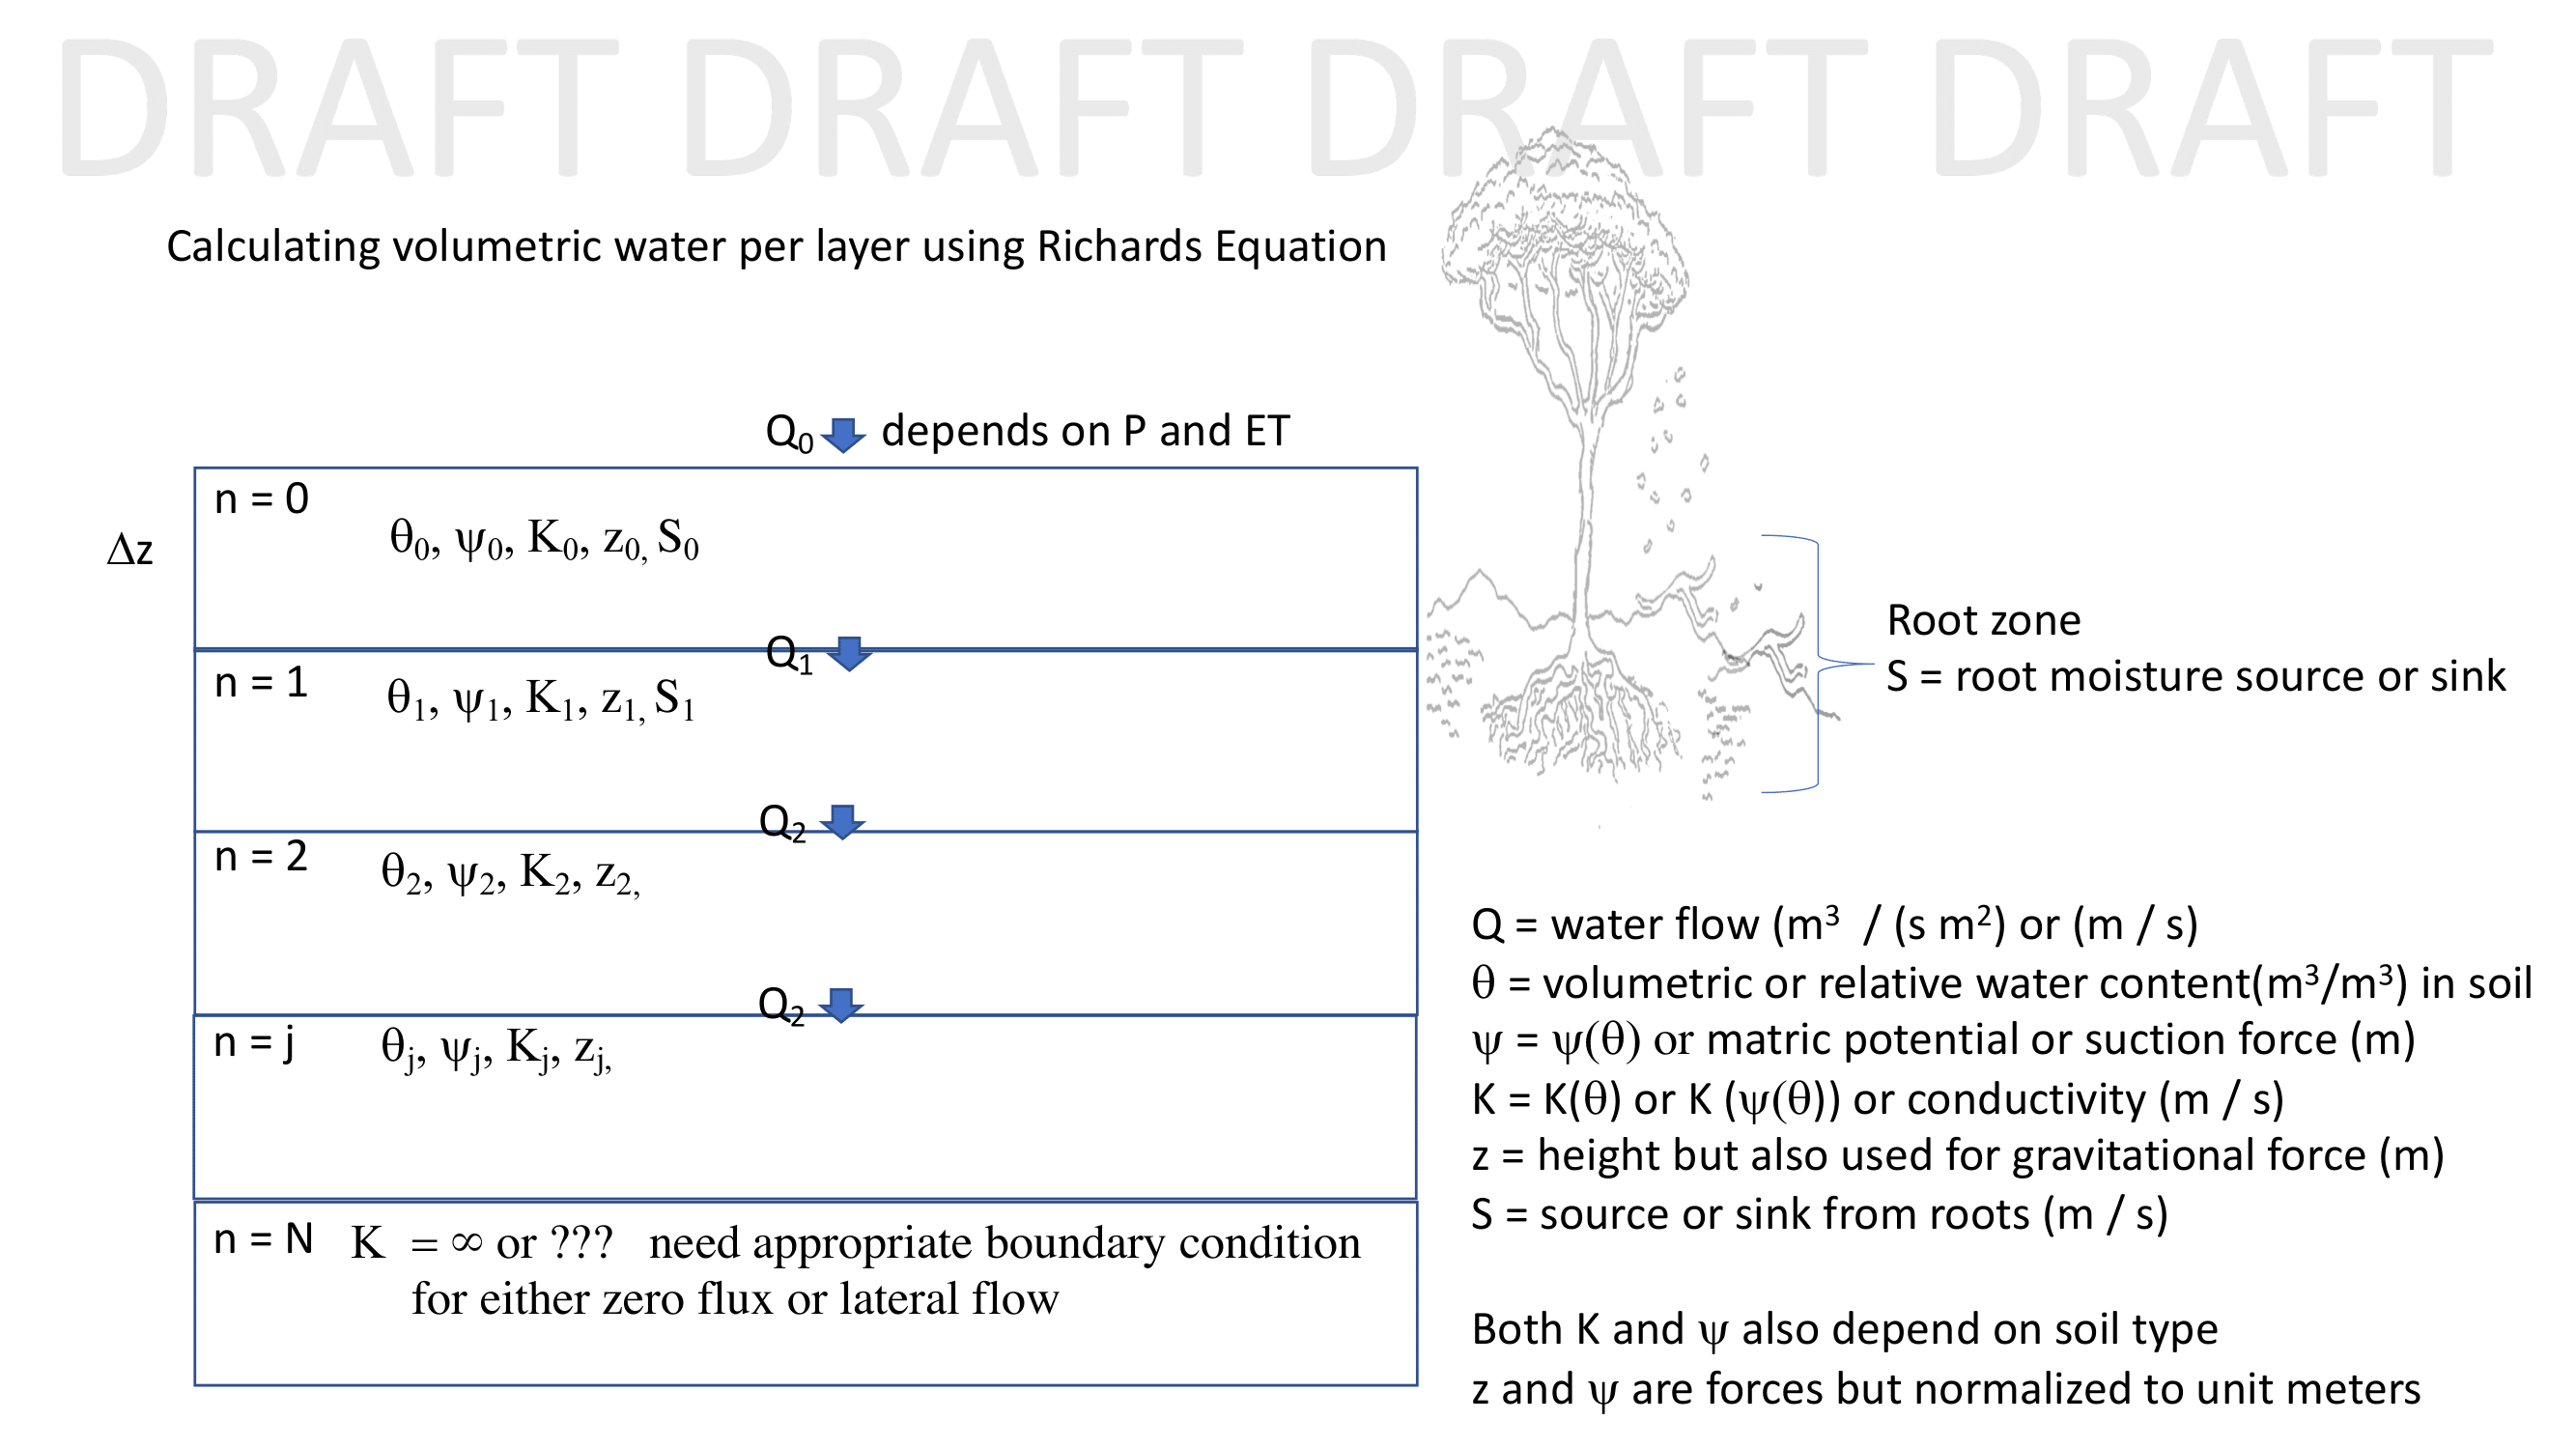
\includegraphics[scale=.15]{CLIMA-land/LM_figures/SoilSchematic-1.png}
\caption{Draft of soil schematic figure}
\end{figure}





\subsection{Moisture equation}
/* Pierre: note that I had not included ice at the time I wrote this - based on the point above it should eb added */
/* very important: people suusally solve this by splitting the domain into an unsaturated and saturated region - the saturated region is then solved in terms of bul avergae propoerties - we could rather solve it as a continuum - this requires some cahnge of thinking - solving for a compressible fluid and matric below the saturation zone. OK with you all? */

Moisture conservation is usually divided into two steps: 1) the unsaturated zone where total water storage is related to the relative water content $\theta$ and transport is typically assumed to be 1D in the vertical and 2) the saturated zone where water storage is related to changes in the water head through the storativity (porosity for an unconfined aquifer, and storativity for confined aquifer), which is treated as a bulk average over the aquifer thickness. 
Let us start with the 3D Richards' equation so we do not lose generality (1D flow is just an approximation similar to shallow water equation). Water storage is written as $S$ (units of $m^3/m^3$). For instance in the unsaturated soil, the storage is related to the water content $S=\theta$. In an unconfined aquifer $dS=S_y dh$, with $S_y$ the unconfined aquifer specific yield, nearly equal to porosity $n$. Finally, in the confined aquifer $dS=S_s dh$, with $S_s$ the aquifer storativity. Note that the concept of aquifer storativity implicitly assumes a vertically-integrated Richards' equation over the thickness of the aquifer $b$. 

Without loss of generality we can therefore write the storage as a (nonlinear) function of the head 
\begin{equation}
     h=z+\psi,
\label{head}
\end{equation}

with $\psi$ the matric potential so that $dS = C(\psi)d\psi$. In the unsaturated case C($\psi$)=$\partial \theta /\partial h$ \\ and in the saturated (unconfined aquifer) case it is the specific yield $C(\psi)=S_y$.
We therefore write the conservation of mass including sinks/sources (such as due to roots but also for instance non-local transport due to preferential flow). 
So the generic 3D Richards' equation using chain's rule:
\begin{equation}
     \frac{\partial S}{\partial t} = C(\psi)\frac{\partial \psi}{\partial t} = -\nabla \cdot {\bf{q}} + {\rm Source}
\label{Richards}
\end{equation}
with $\bf{q}$ Darcy's flow, with 
\begin{equation}
     \bf{q} = - \mathbf{K}(\psi) \otimes \nabla h
\end{equation} with $ \mathbf{K}$ the hydraulic conductivity tensor, and $\otimes$ the tensor product.
For simplicity we will assume that the flow is isotropic and therefore along the head gradient (this might not be true because of the strong horizontal layering of the soil creating important anisotropy; this could be relaxed later):
\begin{equation}
     {\bf{q}} = - K \ \nabla h
\end{equation}
So we are left with our simplified Richards' 3D equation:
\begin{equation}
     C(\psi)\frac{\partial \psi}{\partial t}  = \nabla \cdot \left( {K(\psi) \nabla h} \right) + {\rm Source}
\label{Richards_simple}
\end{equation}
Equation (\ref{Richards_simple}) written in head term is continuous across saturation interfaces.
We finally write this in terms of $\psi$ only
\begin{equation}
     C(\psi)\frac{\partial \psi}{\partial t}  = \nabla \cdot \left( {K \nabla \psi} + K \right) + {\rm Source}
\label{Richards_simple}
\end{equation}


In the unsaturated zone, the storage is simply $S=\theta$, yet we will keep a head-based approach for continuity. $\theta$ is related to $h$ though the so-called retention curves (assuming negligible hysteresis). The potential options for the retention curves are discussed in section \ref{SoilMoisture:Retention_Curves}

Therefore in the unconfined aquifer we will have 
\begin{equation}
     \frac{\partial \theta}{\partial \psi}\frac{\partial h}{\partial t} = \nabla \cdot \left( {K(\psi) \nabla \psi} + K(\psi) \right) + {\rm Source}
\label{Richards_simple_uns}
\end{equation}
This is then solved typically in the vertical and simplifies to:
\begin{equation}
     \frac{\partial \theta}{\partial \psi}\frac{\partial \psi}{\partial t} = \frac{\partial}{\partial z}  \left( {K \frac{\partial \psi}{\partial z} + K(\psi)} \right) + {\rm Source}
\label{Richards_simple_uns_1D}
\end{equation}
with $K(\psi)$, an exponential function of $\psi$.
\st{We note however that as the horizontal resolution becomes finer and in the presence of rain this assumption is not tenable anymore}.
In an unconfined aquifer, below the water table, we will use the bulk average equation integrated over the depth of the aquifer, and the storage over the entire depth is written as a function of the specific yield $S_y$:
\begin{equation}
     \frac{\partial S}{\partial t} = S_y \frac{\partial h}{\partial t}  
\end{equation}
this will lead to the following equation:
\begin{equation}
     \frac{\partial S}{\partial t} = S_y \frac{\partial h}{\partial t} = \nabla \cdot \left( {K_{\rm sat} \nabla h} \right) + {\rm Source}
\label{Richards_simple}
\end{equation}
with $K_{\rm sat}$ the saturated hydraulic conductivity. 


\begin{table}[]
\resizebox{\textwidth}{!}{%
\begin{tabular}{lllll}
\hline
State Variables & Description   & Units     & Range & Example value \\ \hline
$S$       & Water Storage                    & m$^3$/m$^3$ & 0 - 1 & 0.43 m$^3$/m$^3$       \\
$b$       & Aquifer Thickness  & m &  0 - $\infty$  & 10 m        \\


\hline
Auxiliary State Variables & Description   & Units     & Range & Example value \\ \hline
$\theta$       & Relative Water Content                    & m$^3$/m$^3$ & 0 - 1       & 0.2 m$^3$/m$^3$ \\
$\psi$       & Matric Potential  & m or kPa &  $-\infty$ - $\infty$  & 10 m or 100 kPa       \\
$h$       & Hydraulic Head  & m or kPa &  $-\infty$ - $\infty$    & 10 m or 100 kPa     \\
$z$       & Height or Depth & m  &  0 - $\infty$    & 10 m     \\
$\bold{q}$       & Darcy's Flow  & m$^3$/s &  0 - $\infty$   & 1e$^{-6}$ m$^3$/s     \\


\hline
Constants (known) & Description   & Units     & Range & Example value \\ \hline
$S_{y}$       & Unconfined Aquifer Specific Yield   & m$^3$/m$^3$ &  0 - 1   & 0.2 m$^3$/m$^3$     \\
$S_{s}$       & Aquifer Storativity   & m$^3$/m$^3$ &  0 - 1 & 0.25 m$^3$/m$^3$       \\
$K$   & Hydraulic Conductivity &   m/s or cm/day       &    0 - $\infty$ & 0.1 cm/day    \\
$K_{sat}$   & Saturated Hydraulic Conductivity &   m/s or cm/day       &    0 - $\infty$ & 10 cm/day                    \\
$n$       & Porosity   & m$^3$/m$^3$  &   0 - 1  & 0.45 m$^3$/m$^3$     \\


\hline
Constants (empirical) & Description   & Units     & Range & Example value \\ \hline
$\theta_{r}$       & Residual Water Content   & m$^3$/m$^3$ & 0 - 1       & 0.05 m$^3$/m$^3$ \\
$\theta_{s}$       & Saturated Water Content   & m$^3$/m$^3$ & 0 - 1       & 0.45 m$^3$/m$^3$ \\
$\alpha$   & VG Scale Parameter for Retention Function & cm$^{-1}$ & 1e$^{-6}$ - 1e$^{-4}$  & 1e$^{-5}$ cm$^{-1}$ \\
$n$   & VG Shape Parameter for Retention Function & (-) & 4.0 - 8.0  & 7.1 \\
$L$   & VG Empirical Parameter for Retention Function & (-) & 0 - 1  & 0.5 \\
$S_{e}$   & Relative Degree of Saturation of the Soil & (-) & 0 - 1  & 0.25 \\



\hline
\end{tabular}%
}
\caption{List of moisture eqs variables [eventually maybe split into "states" and "parameters" tables]}
\end{table}

\subsubsection{Retention curves $\theta=f(\psi)$ and $K(\psi)$ in the unsaturated zone}
\label{SoilMoisture:Retention_Curves}
    {\bf Van Genuchten} \\
We will use the van Genuchten formulation as a reference retenstion curve, as it is better behaved in saturated conditions than the Brooks and Corey relationship 
\begin{equation}
     \theta(\psi) = \theta_r + \frac{\theta_s - \theta_r}{\left[ 1+(\alpha |\psi|)^n \right]^{m}}
\end{equation}
with $m=1-1/n$.
For hydraulic conductivity, we have
\begin{equation}
     K(\psi) = K_{s} S_e^L \left (1 -  (1-S_e^{1/m})^m  \right)^2
\end{equation}
with $L$ an empirical parameter assumed to be $L=0.5$. $S_e$ is the relative degree of saturation of the soil and $K_{s}$ the hydraulic conductivity at saturation. 
\begin{equation}
     S_e = \frac{\theta(\psi) - \theta_r}{\theta_s - \theta_r}
\end{equation}
The derivative of $\theta$ with respect to $\psi$, $C(\psi)$ is:
\begin{equation}
     \frac{\partial \theta}{\partial \psi} =   \frac{m n\alpha^n |\psi|^{n-1}}{\left[ 1+(\alpha |\psi|)^n \right]^{m+1}} \left( \theta_s - \theta_r \right). 
\end{equation}


    {\bf Brooks and Corey} \\
An alternative approach to Van Genuchten will be to use the Brooks-Corey relationships:
\begin{equation}
     S_e = \frac{\theta(\psi) - \theta_r}{\theta_s - \theta_r} = \left( \frac{\psi}{\psi_{ae}}\right)^{-\lambda}
\end{equation}
with $\psi_{ae}$ the air entry point.
\begin{equation}
     K_s = \left( \frac{\psi}{\psi_{ae}}\right)^{-2-3\lambda}
\end{equation}






\st{Dupuit–Forchheimer assumptions: flow is nearly 2D below the water table (similar to shallow water approximation) and hydrostatic i.e. $\partial h/\partial z=0$.}

\subsection{Summary of soil heat and moisture equations for CliMA implementation}

This section contains a summary of all equations needed for implementation of the soil heat and moisture equations into CliMA. All variables are defined 

[OPTION: list equations in table for succinct description and avoid extra equation numbers in document] \\

\textbf{Soil Heat Equation} \\


\begin{equation}
     \frac{\partial (\rho_s c_s T_s) }{\partial t} = \frac{\partial }{\partial z}\lambda_s \frac{\partial T_s }{\partial z}
\end{equation}

\begin{equation}
    f_{om} = \rho_{om}/\rho_{om,{\rm max}}
\end{equation}


\begin{equation}
\lambda_s = K_e \lambda_{\rm sat} + (1-K_e) \lambda_{\rm dry}
\end{equation}

\begin{equation}
K_e = \exp \big( \gamma((1-s(\gamma-1.33))\big)
\end{equation}

\begin{equation}
s=\theta/\theta_{\rm sat}
\end{equation}

\begin{equation}
c_s=\theta c_{\rm liq} + (1-\theta) c_{\rm dry}
\end{equation}

\begin{equation}
c_{\rm dry} = (1-f_{om})c_{soil} + f_{om}c_{om}
\end{equation}

\begin{equation}
c_{soil} = {\rm \frac{2.128 (sand)+ 2.385 (clay)}{(sand) + (clay)}}
\end{equation}  \\



\textbf{Soil Moisture Equations} \\

(Unsaturated soil)
\begin{equation}
 dS=d\theta 
\end{equation}

(Saturated - Unconfined Aquifer)
\begin{equation}
 dS=S_y dh ; S_y = n
\end{equation}

(Saturated - Confined Aquifer)
\begin{equation}
 dS=S_s dh
\end{equation}

\begin{equation}
 h=z+\psi
\end{equation}

\begin{equation}
dS = C(\psi)d\psi
\end{equation}

(Unsaturated soil)
\begin{equation}
C(\psi)=\partial \theta /\partial h 
\end{equation}

(Saturated  - Unconfined Aquifer)
\begin{equation}
C(\psi)=S_y 
\end{equation}

\begin{equation}
     \frac{\partial S}{\partial t} = C(\psi)\frac{\partial \psi}{\partial t} = -\nabla \cdot {\bf{q}} + {\rm Source}
\label{Richards}
\end{equation}

\begin{equation}
     \bf{q} = - \mathbf{K}(\psi) \otimes \nabla h
\end{equation}

\begin{equation}
     {\bf{q}} = - K \ \nabla h
\end{equation}

\begin{equation}
     C(\psi)\frac{\partial \psi}{\partial t}  = \nabla \cdot \left( {K(\psi) \nabla h} \right) + {\rm Source}
\label{Richards_simple}
\end{equation}

\begin{equation}
     C(\psi)\frac{\partial \psi}{\partial t}  = \nabla \cdot \left( {K \nabla \psi} + K \right) + {\rm Source}
\label{Richards_simple}
\end{equation}

\begin{equation}
     \frac{\partial \theta}{\partial \psi}\frac{\partial h}{\partial t} = \nabla \cdot \left( {K(\psi) \nabla \psi} + K(\psi) \right) + {\rm Source}
\label{Richards_simple_uns}
\end{equation}

\begin{equation}
     \frac{\partial \theta}{\partial \psi}\frac{\partial \psi}{\partial t} = \frac{\partial}{\partial z}  \left( {K \frac{\partial \psi}{\partial z} + K(\psi)} \right) + {\rm Source}
\label{Richards_simple_uns_1D}
\end{equation}

(Saturated - Unconfined Aquifer)
\begin{equation}
     \frac{\partial S}{\partial t} = S_y \frac{\partial h}{\partial t}  
\end{equation}

\begin{equation}
     \frac{\partial S}{\partial t} = S_y \frac{\partial h}{\partial t} = \nabla \cdot \left( {K_{\rm sat} \nabla h} \right) + {\rm Source}
\label{Richards_simple}
\end{equation} \\


\textbf{Retention functions for unsaturated soils - van Genuchten} \\


\begin{equation}
     \theta(\psi) = \theta_r + \frac{\theta_s - \theta_r}{\left[ 1+(\alpha |\psi|)^n \right]^{m}}
\end{equation}

\begin{equation}
m=1-1/n
\end{equation}

\begin{equation}
     K(\psi) = K_{s} S_e^L \left (1 -  (1-S_e^{1/m})^m  \right)^2
\end{equation}

\begin{equation}
L = 0.5
\end{equation}

\begin{equation}
     S_e = \frac{\theta(\psi) - \theta_r}{\theta_s - \theta_r}
\end{equation}

\begin{equation}
     \frac{\partial \theta}{\partial \psi} =   \frac{m n\alpha^n |\psi|^{n-1}}{\left[ 1+(\alpha |\psi|)^n \right]^{m+1}} \left( \theta_s - \theta_r \right) 
\end{equation}


\subsection{Soil properties datasets}
The ISRIC website (https://www.isric.org/explore/soil-geographic-databases) has a long list of soil datasets. A commonly used soil dataset in ESMs is the Harmonized World Soil Database, a 30 arc-second raster database (http://www.fao.org/soils-portal/soil-survey/soil-maps-and-databases/harmonized-world-soil-database-v12/en/) including: organic Carbon, pH, water storage capacity, soil depth, cation exchange capacity of the soil and the clay fraction, total exchangeable nutrients, lime and gypsum contents, sodium exchange percentage, salinity, textural class and granulometry.
 
And a more recent global dataset of soil hydraulic and thermal parameters derived respectively from the Global Soil Dataset for Earth System Models (GSDE) \citep{Shangguan2014} and SoilGrids \citep{Hengl2014,Hengl2017} databases (http://globalchange.bnu.edu.cn/research/soil5d.jsp ). This new dataset is ready to use in CLM (8 soil layers (0 - 0.0451 m, 0.0451 - 0.0906 m, 0.0906 - 0.1655 m, 0.1655 - 0.2891 m, 0.2891 - 0.4929 m, 0.4929 - 0.8289 m, 0.8289 - 1.3828 m, 1.3828 - 3.8019 m)) or JULES (4 soil layers (0 - 0.1 m, 0.1 - 0.35 m, 0.35 - 1.0 m, and 1.0 - 3.0 m)). The spatial resolution is also 30” and includes: volumetric fraction of gravels, volumetric fraction of Soil Organic Matter, volumetric fraction of sand, volumetric fraction of silt, volumetric fraction of clay, volumetric fraction of quartz within mineral soils, saturated water content, log-10 transformation of saturated hydraulic conductivity, saturated suction for the Campbell model \citep{Campbell1974}, pore size distribution index for the Campbell model, residual moisture content for the Van Genuchten  (VG) model \citep{VanGenuchten1980}, the inverse of the air-entry value for the VG model, log-10 transformation of a shape parameter for the VG model, volumetric heat capacity of soil solids in a unit soil volume, thermal conductivity of unfrozen saturated soils, thermal conductivity of frozen saturated soils, and thermal conductivity of dry soils.
 
A global map of bedrock depth up to 250 m can be found in  http://globalchange.bnu.edu.cn/research/dtb.jsp.




\section{Land Boundary conditions}
We first discuss the heat boundary conditions for the soil medium.
\subsection{Ground heat flux at depth}
The bottom boundary condition for the soil will be assumed to be a vanishing ground heat flux $G=0$ at the bottom of the deepest soil layer. This will avoid specifying a constant temperature which would generate an artificial ground heat flux. Initialization will be based on preindustrial annual mean temperature for the soil profile to avoid too long spin up times.

\subsection{Surface energy budget}
The surface heat condition is a mixed boundary condition as it involves resolving the surface energy budget (SEB). The SEB including the canopy air heat capacity can write:
\begin{equation}
    \int_0^h{C_{air}dz \frac{\partial T_{air}(z)}{\partial t}} = R_n - G_0 - H - L_vE - GPP 
\end{equation}
with $C_{air}$ the specific heat of the air, $h$ the vegetation height, $R_n$ the net radiation at the top of the canopy, $G_0$ the ground heat flux at $z$=0, $H$ the sensible heat flux at the top of the canopy, $L_vE$ the latent heat flux at the top of the canopy and $GPP$ gross primary productivity within the canopy (a small but non-negligible term). Note that this neglect heat flux on stems (can be as large as ground heat flux but still need to be explored more carefully).

 The SEB will be solved for the skin temperature at the leaf/soil interface. To do so we will use a multi-layer canopy and a soil layer.
 The total SEB is then split into two components: the soil and canopy ones, allowing the resolution of the vegetation and soil temperatures.
 
\subsubsection{Soil surface energy budget}
The soil SEB is simply:
\begin{equation}
     R_{n,s} - G_0 - H_s - L_vE_s = 0  
     \label{SEB:soil}
\end{equation}
with $R_{n,s}$ the surface soil net radiation, $H_s$ the soil sensible heat flux, and $L_vE_s$ the soil latent heat flux.

\subsubsection{Vegetation surface energy budget}
The vegetation budget in turn is:
\begin{equation}
     R_{n,v} - G_v - H_v - L_vE_v - GPP = 0  
     \label{SEB:veg}
\end{equation}
with $R_{n,s}$ the vegetation net radiation, $H_s$ the vegetation sensible heat flux, $L_vE_s$ the vegetation latent heat flux, and $G_v$ the trunk heat flux, assumed to be negligible. 

At the leaf surface in the canopy, we will use a multi-layer canopy budget
\begin{equation}
    \int_z^{z+\delta z}{C_v (LM_d+S_d) dz\frac{\partial T_v}{\partial t}} = R_{n,v}(z) -H_v(z)-L_vE(z)-GPP(z)
\end{equation}
with $LM_d$ the mass vertical density of leaves, related to the leaf mass area and therfore to the lead area index density $LAId$, and leaf specific mass $LM$. $S_d$ is the stem mass vertical density.
(Note that the atmosphere will have to see the sensible and latent heat fluxes but we leave the atmosphere component as part of the atmospheric module). Note importantly that the canopy is considered as a dense canopy, i.e. like a porous medium so not all space can be filled up with air because of the stems and canopy volume. This will require some correction factor in the mass and energy conservation in the atmosphere at the top of the canopy for continuity (Schmid et al., 2019).

\subsection{Surface evapotranspiration}
Surface evapotranspiration is composed of four terms: 1. open-water body evaporation (e.g. lakes), 2. soil evaporation, 3. Plant canopy transpiration and 4. Canopy interception
\subsubsection{Open-water evaporation}
The open water body evaporation will simply use the same formulation as the ocean model (including waves).
\subsubsection{Soil evaporation}
Soil evaporation modeling has typically been relatively empirical leading to systematic issues with soils either drying much too fast or too slowly. We here use a recent formulation (Lehmann et al., 2019) informed by observations from either laboratory or in situ flux observations (Merlin et al. 2018). This formulation is aimed at modeling the evaporative front and its impact on soil evaporation. 
Soil evaporation then is 
\begin{equation}
    E_s = \rho \frac{e_s(T_s)-e_{a,s}}{r_{a,s}+r_{\rm shell}+r_{\rm soil}}
\end{equation}
with $e_{a,s}$ the near surface air vapor pressure, $r_{a,s}$ the surface aerodynamic resistance between the surface and near surface level, composed of a viscous boundary layer resistance $\delta /D_{air}$, with $\delta$ the depth of the viscous boundary layer (note that reality is trickier with a buffer regime - matching the viscous and turbulent layers). It should not be a major issue as this resistance will typically not be the primary limitation. The vapor shell resistance $r_{\rm shell}$ is due to the configurational resistance to diffusion through vapor shells forming around evaporating pores i.e. diffusion in 3-D from the evaporating pores across a hemisphere (Bange, 1953; Schlünder, 1988).
\begin{equation}
    r_{\rm shell} = \frac{1}{D_{\rm air}}\frac{\overline{r_{\rm pore}}(\pi-2\sqrt{\theta(z=0)})}{4\theta(z=0)}
\end{equation}
with mean pore size $\overline{r_{\rm pore}}$.
The soil resistance is related to the evaporative font and Darcy's law of capillarity effects.
\begin{equation}
    r_{\rm soil} = \frac{1}{4 K_s(\theta(z=0))\frac{\Delta H}{\Delta Z}}\frac{e_s(T_s)-e_{a,s}}{\rho}
\end{equation}
with $\frac{\Delta H}{\Delta Z}$ the head across a layer $\Delta Z$ (surface acppilarity effects between the wet subsurface and dry surface). It can be shown that (Lehmann et al., 2008; 2019) that 
\begin{equation}
   \frac{\Delta H}{\Delta Z} = \frac{L_{\rm gravity}}{L_{\rm capillarity}} = 1+E_0/(4K_s(h_c))
\end{equation}
with $E_0$ thes surface potential evaporation (i.e. in the absence of shell and soil resistances) “gravity length” $L_{\rm gravity}$ (difference between air entry value $h_b$ and critical capillary pressure head $h_c$ at which hydraulic flow paths become disconnected) with $h_c$ obtained from van Genuchten as:
\begin{equation}
   h_c = \frac{1}{\alpha}\left( \frac{n-1}{n} \right)^{\left( \frac{1-2n}{n} \right)}
\end{equation}

\subsubsection{Canopy reevaporation}
Interception of rainwater by the canopy remains highly empirical and few parameterizations exist. Those parameterization are not physically based and were tested at only very few sites. We are currently developing a method that should be able to give much better estimates of rainfall interception using hybrid machine leaning approaches, showing a clear dependence on rainfall maximum and Leaf Area Index. FOR LATER

\subsubsection{Transpiration}
Transpiration will follow an approach based on optimal stomatal behavior, which assumes that stomata are maximizing carbon uptake while minimizing water losses through transpiration (see photosynthesis section). 
Since we will use a multi-layer canopy we will always consider as the air reference value, the air in the vicinity of the leaves and thus at the same height $z$. We note that the air resistance should not be defined based on Monin-Obukhov Similarity Theory (MOST) but is rather due to von Kármán vortex streets.
The transpiration at level $z$ will be
\begin{equation}
    E_l = LAI_d \ \rho \frac{e_s(T_l(z))-e_{a}(z)}{r_{a,v}(z)+r_{\rm sto}(z)}
\end{equation}
Pierre: Note I placed $LAI_d$ in front of $E_l$ to emphasize that it is the density of leaves that is generating transpiration. Another choice would have been to have it dividing $r_{\rm sto}(z)$ but since turbulence is also due to the leaves it is more convenient to have it in font of everything as a density weigthing (easier to integrate).

\subsection{Ground heat flux at depth}
\subsubsection{Infiltration excess runoff}
At the surface during high-rainfall events, the rate of precipitation can exceed that of infiltration. This is modeled very simply as an infiltration excess (i.e. Hortonian runoff). The excess rate $i_H = P_s-q(z=0)$ is then directly assumed to run off into the streams. Note that it requires fine time stepping.

\subsubsection{Saturation excess runoff}
When the infiltration exceeds the saturation capacity, the residual is assumed to also run off (Dunne runoff). This is quite simple: withing a time step if soil moisture at any level in the soil column exceeds saturation, the residual is assumed to run off into the stream. This mechanism generally occurs near the stream where the water table is higher. We note that the landscape is prescribed and could be based on a DEM. 

\subsubsection{Groundwater baseflow}
The horizontal gradient of water in the landscape is continuously feeding the stream and is related to the horizontal gradient of $\mathbf{q}$: $-\nabla_H \cdot \mathbf{q}$.

\subsubsection{Streams}
Runoff will be channeled into the CaMa Flood model.

\begin{itemize}
\item Dissolved organic carbon in runoff $\mathrm{= NBP = GPP - R_{eco} - fire - disturbance}$. So, DOC in runoff can constrain NBP.

\item Model CO2 in soil
\item Need deep soil (tens of layers, extending over ~200 m)
\end{itemize}

\section{Snow}

Model bulk snow water equivalent, close energy and water budgets.

AABLOOM: empirical parametrization for \% snow cover? Should be independent of bulk snow energy + water budgets, but will directly impact surface albedo (?).

\section{Vegetation}

%Multi-layer canopy model

%Include tracers such as 13C, OCS

The vegetation model is based on the mSCOPE model \citep{Yang2017}, where leaf spectral properties are calculated based on the PROSAIL framework \citep{Jacquemoud2009} and photosynthesis as in \citet{Farquhar1980}. The RTM simulates the light distribution within the canopy, while the photosynthesis model simulates the energy partitioning in photosystems.

The model mSCOPE includes a vertically heterogeneous vegetation canopy. It follows the same principle of SCOPE \citep{VanderTol2009}, that simulates the spectrum of top of the canopy reflected radiation, fluorescence emission in the viewing direction, and photosynthesis as functions of leaf properties, vegetation structure, and micrometeorological conditions. %Leaf and canopy radiative transfer schemes combined with an energy balance model.%
At leaf level, Fluspect \citep{Vilfan2016} is used to simulate leaf reflectance, transmittance, and fluorescence. At canopy level, RTM$_{optical}$ and RTM$_{fluorescence}$ \citep{VanderTol2016}, which are two SAIL \citep{Verhoef1984,Verhoef1985} based models, compute the radiative transfer of incident radiation and emitted fluorescence, respectively. 

To overcome the assumption of homogeneity in the horizontal direction made in mSCOPE, this new version incorporates a parameterization scheme of horizontal structural heterogeneity following SPARTACUS-Vegetation 1.1 \citep{Hogan2018}.

\subsection{Radiative transfer}

%Let radiation (spectrally resolved) interact with canopy.

%Use Monte-Carlo Independent Column Approximation (ICA) to sample from canopy/soil properties, at the same time as sampling from cloud properties (no marginal cost); need assumed distribution of leaf area index to sample

%\subsubsection{The PROSAIL Model}%

PROSAIL combines the leaf optical properties of the model PROSPECT \citep{Jacquemoud1990,Feret2017} with the turbid medium canopy radiative transfer model SAIL. The models are coupled so that the simulated leaf reflectance and transmittance from PROSPECT are fed into the SAIL model, completed with information about soil optical properties and illumination/observation geometry.

 Extra input parameters of mSCOPE compared with SCOPE include an explicit definitition of LAI and leaf properties per canopy layer. Leaf properties parameters include $C_{ab}$, $C_{dm}$, $C_{w}$, $C_{s}$, $C_{ca}$ and $N$. The main input variables of the integrated model are shown in the Table \ref{tab:prosail}.

\begin{table}[]
\resizebox{\textwidth}{!}{%
\begin{tabular}{llllll}
\hline
Model & Symbol   & Description     & Unit & Range & Example value\\ \hline
PROSPECT  & $N$                    & Leaf structure parameter &  - & 1 - 3 & 1.5\\
  & $C_{ab}$                    & Chlorophyll a + b content &  $\mu$g cm$^{-2}$ & 0 - 100 & 40      
       \\
    & $C_{dm}$                    & Leaf mass per unit area &  g cm$^{-2}$  & 0 - 0.02 & 0.01     
       \\      
   & $C_{w}$                    & Equivalent water thickness &  cm  & 0 - 0.05 & 0.015   
       \\
   & $C_{m}$                    & Dry matter content &  g cm$^{-2}$ & 0 – 0.5 & 0.012      
       \\
    & $C_{s}$                    & Senescence material (brown pigments)  &  fraction  & 0 – 1 & 0.1    
       \\
  & $C_{ca}$                    & Caratenoid content  &  $\mu$g cm$^{-2}$  & 0 – 30 & 10      
       \\
\hline
SAIL  & $LAI$                    & Leaf area index &  m$^2$.m$^{-2}$ & 0 – 6 & 3       \\
   & $LIDF_{a}$                    & Leaf inclination distribution function parameter a &  - & -1 – 1 & -0.35       \\
   & $LIDF_{b}$                    & Leaf inclination distribution function parameter b &  -  & -1 – 1 & -0.15        \\ 
  & $s_{L}$                    & Hot spot parameter &         \\
  & $\rho$$_{s}$                    & Soil reflectance assumed Lambertian or not &  -        \\
    & $SKYL$                    & Ratio of diffuse to total incident radiation &  -  & 0 - 1 & 0.42      \\
    & $sza$ or $\theta_{s}$               & Solar zenith angle &  deg & 0 - 90 & 45       \\
    & $vza$ or $\theta_{v}$               & Viewing zenith angle &  deg  & 0 - 90 & 45      \\
    & $raa$ or $\phi_{sv}$               & Relative azimuth angle &  deg & 0 - 180 & 90       \\
\hline
  FLUSPECT & $\epsilon$$_{1}$                    & Fluorescence efficiency of photosystem I &  -  & 0 – 0.01 & 0.004   \\
 & $\epsilon$$_{2}$                    & Fluorescence efficiency of photosystem II &  -  & 0 – 0.05 & 0.02      \\

\hline
\end{tabular}%
}
\caption{Main variables of PROSAIL. Adapted from \citet{Jacquemoud2009,Yang2017}}
\label{tab:prosail}
\end{table}

\subsection{Leaf photosynthesis}







\section{River network}
https://agupubs.onlinelibrary.wiley.com/doi/epdf/10.1029/2019WR024873

\bibliographystyle{agufull08}
\bibliography{Renato_refs,CLIMA-refs}

\end{document}
